\documentclass[12pt,a4paper,english]{paper}
\usepackage{fontspec}
\usepackage[T1]{fontenc}
\usepackage[utf8]{inputenc}
\usepackage[left=0.65in,right=0.65in,top=2cm,bottom=1in]{geometry}
\usepackage{multirow}
\usepackage{hyperref}
\usepackage{graphicx}
\usepackage{bm}
\usepackage[usenames,dvipsnames]{color}
\usepackage{booktabs}
\usepackage{fancyhdr}
\usepackage[most]{tcolorbox}
\usepackage{changepage}
\usepackage[square,sort,comma,numbers]{natbib}
\usepackage{amsmath}
\usepackage{amssymb}
\usepackage{eucal}
\usepackage[]{minted}
\usepackage{latexsym}
\usepackage{indentfirst}
\usepackage[ruled,vlined]{algorithm2e}
\usepackage[english]{babel}
\usepackage[autostyle, english = american]{csquotes}
\usepackage[default]{lato}
\usepackage{FiraMono}
\usepackage{lipsum}

\MakeOuterQuote{"}

\def \courseNumber {CS6630}
\def \courseName {Secure Processor Microarchitecture}
\def \assignmentName {Assignment 1}
\def \myName {Arjun Menon V, Akilesh Kannan}
\def \rollNumber {EE18B104, EE18B122}

\setlength{\headheight}{14pt}

\pagestyle{fancy}
\fancyhf{}
\rhead{\assignmentName}
\lhead{\courseNumber: \courseName}
\cfoot{\thepage}

% \linespread{1.2}

\definecolor{blue(ryb)}{rgb}{0.01, 0.28, 1.0}
\definecolor{green(ryb)}{rgb}{0.28, 1.0, 0.01}
\definecolor{red(ryb)}{rgb}{1.0, 0.01, 0.28}
\definecolor{black(ryb)}{rgb}{0, 0, 0}
\definecolor{gray(ryb)}{rgb}{0.75, 0.75, 0.75}
\definecolor{orange}{RGB}{255,155,0}
\definecolor{formalblue}{rgb}{0.95,0.95,1}
\definecolor{formalred}{rgb}{1,0.95,0.95}

\newenvironment{colorboxed}[4][gray]{
\begin{tcolorbox}[colback=#1!3!white,colframe=#1(ryb)!50!black,title=\textbf{#2 #3},#4]
}{
\end{tcolorbox}
}

\newenvironment{warning}{%
  \def\FrameCommand{%
    \hspace{1pt}%
    {\color{red}\vrule width 2pt}%
    {\color{formalred}\vrule width 4pt}%
    \colorbox{formalred}%
  }%
  \MakeFramed{\advance\hsize-\width\FrameRestore}%
  \noindent\hspace{-4.55pt}% disable indenting first paragraph
  \begin{adjustwidth}{7pt}{}%
  \vspace{2pt}\vspace{2pt}%
}
{%
  \vspace{2pt}\end{adjustwidth}\endMakeFramed%
}

\newenvironment{results}{%
  \def\FrameCommand{%
    \hspace{1pt}%
    {\color{blue}\vrule width 2pt}%
    {\color{formalblue}\vrule width 4pt}%
    \colorbox{formalblue}%
  }%
  \MakeFramed{\advance\hsize-\width\FrameRestore}%
  \noindent\hspace{-4.55pt}% disable indenting first paragraph
  \begin{adjustwidth}{7pt}{}%
  \vspace{2pt}\vspace{2pt}%
}
{%
  \vspace{2pt}\end{adjustwidth}\endMakeFramed%
}

\begin{document}
\thispagestyle{empty}
\vspace{-4.5cm}

\hspace*{-\parindent}
\begin{minipage}{0.65\textwidth}
\fontsize{22pt}{10pt}\selectfont\textbf{\assignmentName}\\[1mm]
\Large
\textit{\courseNumber: \courseName}\\[5mm]
\Large \myName \\[1mm]
\normalsize \rollNumber \\
\end{minipage}\hfill% push everything to the right
\raisebox{-13mm}{
\includegraphics[scale=.28]{logo.pdf}}

\hrule \hrule
\medskip

\section{CLEFIA}

\begin{warning}
The CLEFIA-128 cipher implemented here is adapted from the reference implementation provided by SONY Corporation from \href{https://www.sony.net/Products/cryptography/clefia/}{here}.
\end{warning}

\subsection{Approach}
The \texttt{F0} and \texttt{F1} functions in CLEFIA have been implemented using lookup tables (T-Tables). These functions formed the core of CLEFIA, with a \textit{substitution} layer and a \textit{diffusion} layer.

However, due to the diffusion layer, which involves modular arithmetic in \texttt{GF(2$^\text{8}$)}, timing attacks can be done, due to the if-else structure of the multiplication operation in the reference implementation.

To overcome this, we can use lookup tables to perform the F-functions (as well as the following \texttt{XOR} operation), which will occur in constant time\footnotemark.

\footnotetext{Assuming, the table is fully located in cache.}

We have used 8 lookup tables (8KB each) totally to implement the \texttt{F0} and \texttt{F1} functions. This can be reduced to 4 tables, with the other 4 being just a circularly shifted version of these, but we chose not to for the sake of easier understanding.

\begin{colorboxed}{\texttt{F0}, \texttt{F1} functions}{}{breakable}
    \inputminted[baselinestretch=0.85,breaklines,firstline=367,lastline=401,fontsize=\footnotesize]{c}{CLEFIA/src/clefia.c}
\end{colorboxed}

In the above code snippet, the \texttt{TF**} are the lookup tables - the first digit denotes which of \texttt{F0} or \texttt{F1} it is used in and the second denotes which byte of the output it is used for. We perform an endian-ness switch\footnotemark\ in order to make it compatible with the reference implementations' \texttt{XOR} function.

\footnotetext{This is not required in a big-endian machine. Code was tested only on little-endian machines.}

\subsection{Results}
\begin{figure}[H]
    \centering
    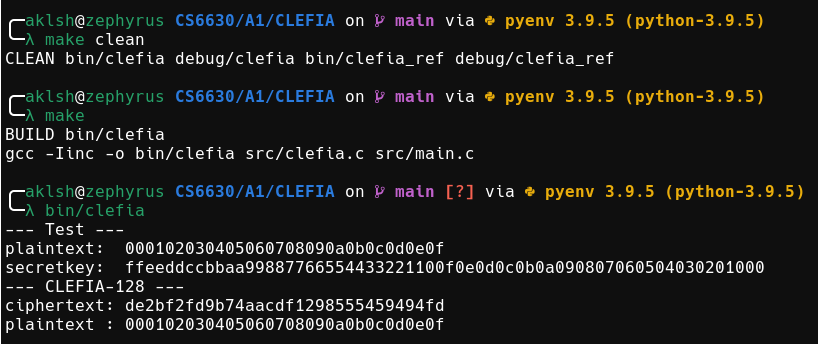
\includegraphics[scale=0.4]{Q1_output.png}
    \label{fig:clefia_cipher}
    \caption{CLEFIA-128 Cipher Output}
\end{figure}

\section{Hashed Password Cracking}
\subsection{Approach}
The following observations were made about the hash implementation:
\begin{itemize}
    \item The hash only used the first \texttt{PRIME} characters of the input password. The rest of the characters didn't matter. This allows one to perform collision attacks on the hash, if the secret key was more than \texttt{PRIME} characters long - all the attacker has to do is to find the first \texttt{PRIME} characters in the secret key.
    \item Each character in the hashed string was dependent only on a single character from the input string. This allows one to easily reverse-engineer the hash by sequentially brute-forcing each of the characters in the correct order as they were used by the hashing mechanism. This reduced the number of tries exponentially - from \texttt{PRIME}$^\text{N}$ to \texttt{PRIME}$*\text{N}$, where N is the number of characters in the search space.
\end{itemize}

Based on these observations, we wrote a python script that starts with a known password (the blank password), and sequentially try brute-forcing the characters in the correct order as used by the hash. The correct character can be identified by a spike in the time taken for the hash computation (will increase by 1 sec). The next iteration of the cracker will use this character and try guessing the next character.

In order to automate this process, we used TCP sockets to communicate with the server.

\begin{colorboxed}{Password cracker script}{}{breakable}
    \inputminted[baselinestretch=0.85,breaklines,fontsize=\footnotesize]{python}{HashCollision/cracker.py}
\end{colorboxed}

\subsection{Results}

\begin{table}[H]
\centering
\begin{tabular}{@{}cc@{}}
\toprule
\textbf{Parameter}           & \textbf{Value}                 \\ \midrule
\multicolumn{1}{c}{Password} & \texttt{spm\{fastandfurious\}}  \\ \midrule
\multicolumn{1}{c}{Guesses}  & 153                             \\ \midrule
\multicolumn{1}{c}{\multirow{6}{*}{Colliding passwords}} & \texttt{spm\{fastandfurious\}\_hacked}              \\ \cmidrule(l){2-2}
\multicolumn{1}{c}{}                                     & \texttt{spm\{fastandfurious\}\_h4ckeD}  \\ \cmidrule(l){2-2}
\multicolumn{1}{c}{}                                     & \texttt{spm\{fastandfurious\}c011iDe}   \\ \cmidrule(l){2-2}
\multicolumn{1}{c}{}                                     & \texttt{spm\{fastandfurious\}\_c0lliDe} \\ \cmidrule(l){2-2}
\multicolumn{1}{c}{}                                     & \texttt{spm\{fastandfurious\}\_fA5t9} \\ \bottomrule
\end{tabular}
\caption{Summary}
\label{tab:summary}
\end{table}

\begin{figure}[H]
    \centering
    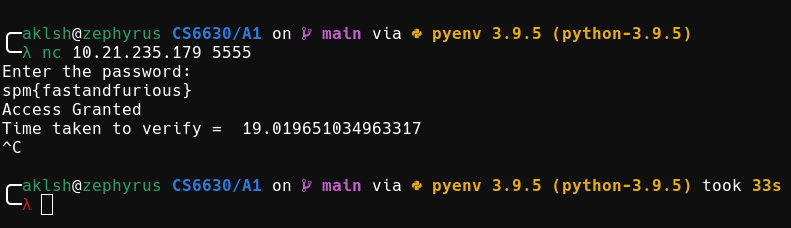
\includegraphics[scale=0.4]{Q2_output.png}
    \label{fig:output_password}
    \caption{Password cracked and access granted}
\end{figure}



%Beginning References. Don't add any text beyond this.
%------------------------------------------

%\newpage %sending References to the last page

\bibliography{paper}
\bibliographystyle{acm}
\end{document}
